\chapter{Lichtbrechung in der Atmosph"are\label{chapter:thema}}
\lhead{Lichtbrechung in der Atmosph"are}
\begin{refsection}
\chapterauthor{Simon Schaefer und Tibor Schneider}

\printbibliography[heading=subbibliography]
\end{refsection}

%polar plot
\usepgfplotslibrary{polar}

\section{Einleitung}
Der Blick an den Nachthimmel fasziniert uns Menschen schon seit Jahrtausenden. "Ahnlich der Frage "uber das Leben nach dem Tod wurden damit ganze Religionen und Kulturen begr"undet beziehungsweise zugrunde gerichtet. 
"Uber die Jahrhunderte wuchs die Einsicht, wenn auch nicht stetig und leider auch nicht strikt monoton, dass eine genauere Vermessung des Nachthimmels, die Astrometrie, wenigstens physikalische Grundlagen zur Diskussion betragen kann. 
W"ahrend Galileo Galilei noch mit blossem Auge und einem besseren Flaschenboden den Nachhimmel beobachtete (TODO: QUELLE), nutzte T. Brahe bereits ein XXX Teleskop (TODO: QUELLE). 
Beide beobachteten die Bewegungen der Planeten unseres Sonnensystems und nahmen die Positionen entfernterer Sterne, Galaxien und anderen Objekten als sogenannte Fixsterne als konstant an. 
W"ahrend die Nasa und andere noch daran t"ufteln einen Menschen auf unseren n"achsten Nachbarplaneten zu bugsieren, sind unsere Blicke und v.a. unsere Neugier bereits Milliarden von Lichtjahren "uber unser Sonnensystem hinaus ins Weltall gerichtet. 
Die ehemaligen Fixsterne sind zu dynamischen Konstallationen erstaunlicher Ph"anomene geworden.
Neue Technologien der Sensorik erz"ahlen uns von der materiellen Zusammensetzung leuchtender Gaswolken. 
Gewaltige Pulsare werden zu Meilensteinen intergalaktischen Kartographie. 
Die Bewegung und die unfassbaren Distanzen ganzer Galaxien von unserem Heimatplaneten geben uns sogar die M"oglichkeit in der Zeit zur"uck zu blicken.
Die Gr"osse unseres Universums  erlaubt es sogar Annahmen "uber das Schicksal unseres eigenen Sonnensystems zu treffen, indem wir andere Systeme beobachten. 
Die extremen Distanzen zwischen uns und den beobachteten Objekten fordern eine hohe Pr"azision bei der Konstruktion der verwendeten Messinstrumente sowie ein tiefes Verst"andnis aller mo"glichen Effekte, die unseren Blick in die Tiefe des Weltalls beeinflussen. 
Angefangen bei simplen Regenwolken, "uber die Lichtverschmutzung unserer Zivilisation, zu optischen Effekten der Lichtbrechung in der Atmosph"are durch die Temperatur und Zusammensamensetzung, ja sogar Bewegung der Lufschichten bis hin zu relativistischen Effekten (TODO: QUELLE), die einen Lichtstrahl aus weiter Ferne so manipulieren k"onnen, dass uns dessen Ursprung an ganz anderem Ort erscheint, als er tats"achlich ist. 
Schon in der Primarschule lehr der Strahlensatz, dass schon kleine Messfehler bei der Auswertung eines Bildes hier auf der Erde, hochgerechnet auf die Weiten des Universums extreme Dimensionen annehmen. (TODO: HISTORISCHES BEISPIEL). 
In diesem Artikel m"ochten wir nun basierend auf Jean Kovalevsky und P. Kenneth Seidelmanns 6. Kapitel in Grundlagen der Astrometrie \cite{licht:astrometry} die scheinbare Verschiebung beobachteter Objekte und deren mathematischen Korrektur beschreiben. 

\section{Planares Modell}
\begin{figure}
\centering
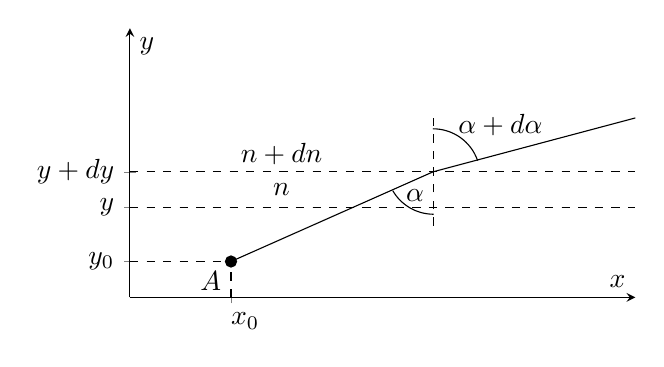
\begin{tikzpicture}
  \begin{axis}[xlabel=$x$, ylabel = $y$, axis lines=middle, height=5cm, width = 8cm,
  ymin=0, ymax=1.5, xmin=0, xmax=1, yticklabels={$y_0$, $y$, $y + dy$}, ytick =
  {0.2,0.5,0.7}, xtick={0.2}, xticklabel={\rlap{$x_0$}}]
    \draw[dashed] (axis cs:0,0.5) -- (axis cs:1,0.5);
    \draw[dashed] (axis cs:0,0.7) -- (axis cs:1,0.7);
    \draw[dashed] (axis cs:0,0.5) -- (axis cs:1,0.5);
    \draw[dashed] (axis cs:0.2,0) -- (axis cs:0.2,0.2);
    \draw[dashed] (axis cs:0,0.2) -- (axis cs:0.2,0.2);
    \filldraw (axis cs:0.2,0.2) circle (2pt) node[anchor=north east] {$A$};
    \draw (axis cs:0.2,0.2) -- (axis cs:0.6,0.7);
    \draw (axis cs:0.6,0.7) -- (axis cs:1,1);
    \draw (axis cs:0.52, 0.595) arc (210:270:0.6cm) node[anchor=north east, yshift =
    +0.44cm] {$\alpha$};
    \draw (axis cs:0.688,0.762) arc (19:90:0.6cm) node[anchor=west, yshift=+0.05cm,
    xshift=+0.2cm] {$\alpha + d\alpha$};  
    \draw[dashed](axis cs:0.6,0.4) -- (axis cs:0.6,1);
    \draw (axis cs:0.3, 0.6) node {$n$};
    \draw (axis cs:0.3, 0.8) node {$n + dn$};
  \end{axis}
\end{tikzpicture}
\caption{Skizze des planaren Modells}
\label{fig:13_1}
\end{figure}


Es wird von der Snell's Gleichung ausgegangen: $n_1 \sin \alpha_1 = n_2 \sin \alpha_2$.
Durch Einsetzen der Oberen Grafik ergibt sich:

\begin{equation} \label{eq:13_1}
  n \cdot \sin(\alpha) = n_0 \cdot \sin(\alpha_0) = \varepsilon
\end{equation}

Aus der Geometrie in der Abbildung \ref{fig:13_1} ist ersichtlich:
$$\frac{\cos \alpha}{\sin \alpha} = \frac{dy}{dx} = y'(x)$$
$$\Rightarrow y'(x)^2 = \frac{1 - \sin^2 \alpha}{\sin^2 \alpha} = \frac{1}{\sin^2 \alpha} - 1$$

Nun k"onnen wir das nach $sin^2(\alpha)$ aufl"osen, indem wir durch $y'(x)^2$ teilen. 
Da diese Ableitung m"oglicherweise $=0$ sein kann, muss dieser Fall separat behandelt werden (siehe Kapitel \ref{ch:spezialfall}). 
Von nun an gilt die Bedingung: $f'(x) \neq 0$.

\begin{equation} \label{eq:13_2}
\sin^2 (\alpha) = \frac{1}{y'(x)^2 + 1}
\end{equation}

Nun quadrieren wir die Gleichung \ref{eq:13_1}, setzen \ref{eq:13_2} ein und l"osen nach $y'(x)$ auf:

\begin{equation} \label{eq:13_3}
n^2 \cdot \frac{1}{y'(x)^2 + 1} = \varepsilon^2 = (n_0 \cdot \sin \alpha_0)^2
\end{equation}

\begin{equation} \label{eq:13_4}
\Rightarrow y'(x)^2 = \left( \frac{n}{\varepsilon} \right)^2 - 1
\end{equation}

Nun k"onnte man die Differentialgleichung nummerisch l"osen. 
Das problem ist aber, dass eine Differentialgleichung zweiter Ordnung vorliegt, jedoch in der Funktion die Anfangssteigung $y'(0)$ (in der Form von $\sin \alpha_0$) vorkommt. 
Dies wird in Kapitel \ref{ch:korrektur} genauer erkl"art.

\subsection{Korrektur der Differentialgleichung} \label{ch:korrektur}

Wie in der Gleichung \ref{eq:13_3} zu erkennen ist, ist der Anfangswinkel in der Gleichung vorhanden. 
Dieser ist von der Anfangssteigung abh"angig. 
Da jedoch die Differentialgleichung (aktuell) in der ersten Ordnung ist, wird die Gleichung \ref{eq:13_3} nach $x$ abgeleitet:

$$\frac{d}{dx} \left( \frac{n^2}{y'^2 + 1} \right) = \frac{2n}{y'^4 + 2y'^2 + 1} \cdot \left( n'(y'^2 + 1) - n y' y'' \right) = 0$$

Nun sind wir $\alpha_0$ losgeworden und haben die jetzt vorliegende Gleichung hat Ordnung 2. 
Nun k"onnen wir den Anfangswinkel $\alpha_0$ als Steigung in den Anfangsbedingungen definieren. 
Da der ganze Term gleich 0 ist, muss der Ausdruck in den Klammern gleich 0 sein:

$$n'y'^2 + n' - n y' y'' = 0$$
$$y''(x) = \frac{n'(y(x))}{n(y(x))} \cdot \left( y'(x) + \frac{1}{y'(x)} \right)$$

Aufgrund der Kettenregel $\frac{dn}{dx} = \frac{dn}{dy} \cdot \frac{dy}{dx}$ kann man die Differentialgleichung weiter vereinfachen:

\begin{equation} \label{eq:planar_DGL}
y''(x) = \frac{\frac{dn}{dy}}{n(y)} \cdot \left( y'(x)^2 + 1\right)
\end{equation}

Als erste approximation verwenden wir $n(y) = 1 + \mu e^{-\sigma y}$ und $\frac{dn}{dy} = -\sigma \mu e^{-\sigma y}$.
Somit sieht die Differentialgleichung folgendermassen aus:

\begin{equation} \label{eq:planar_DGL_n}
y''(x) = \frac{-\sigma}{\frac{1}{\mu e^{-\sigma y}} + 1} \cdot \left( y'(x)^2 + 1 \right)
\end{equation}

\subsection{Spezialfall: $y'(x) = 0$} \label{ch:spezialfall}

An diesem Punkt ist die Funktion $y(x)$ konstant. 
In diesem planaren Modell nimmt die Brechzahl $n$ nur in y-Richtung zu (ist also bei konstantem $y(x)$ ebenfalls konstant).
Aus der Gleichung \ref{eq:13_1} ist ersichtlich, dass bei konstantem $n$ sich das Licht nicht bricht. 
Deshalb wird der Spezialfall folgendermassen behandelt:

$$n' (y'^2 + 1) - n y' y'' = 0$$

Wie erkennbar ist, k"onnen im Fall $y'(x) = 0$ die Funktionen $y(x)$ und $y''(x)$ gew"ahlt werden. 
Ab dem Zeitpunkt $x_0$, bei welchem gilt: $y'(x_0) = 0$, wird die Funktion $y(x)$ folgendermassen definiert:

$$y'(x_0) = 0 \longrightarrow y''(x \geq x_0) = 0, \quad y''(x \geq x_0) = 0, \quad  y(x \geq x_0) = y(x_0)$$


\begin{figure}
\centering
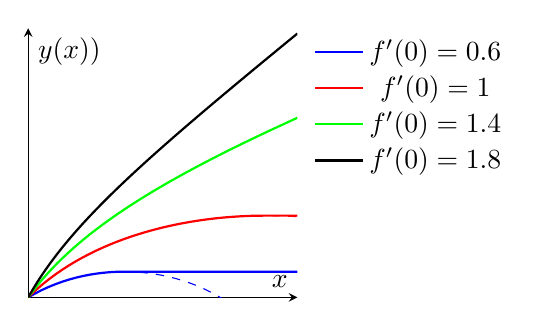
\begin{tikzpicture}
  \begin{axis}[xlabel=$x$, ylabel=$y(x))$, axis lines=middle, height=5cm, width=5cm, ticks
  = none, legend pos = outer north east, legend style={draw=none}, ymin = 0, ymax = 10,
  xmin = 0, xmax = 10] 
  
  \addplot [mark = none, thick, draw=blue] coordinates{
        (0.00000,0.00000)(0.00008,0.00005)(0.00017,0.00010)(0.00025,0.00015)
        (0.00033,0.00020)(0.00075,0.00045)(0.00117,0.00070)(0.00159,0.00095)
        (0.00201,0.00121)(0.00410,0.00246)(0.00620,0.00371)(0.00829,0.00496)
        (0.01038,0.00622)(0.02085,0.01245)(0.03131,0.01866)(0.04178,0.02485)
        (0.05225,0.03100)(0.10458,0.06137)(0.15691,0.09107)(0.20924,0.12012)
        (0.26157,0.14852)(0.51157,0.27569)(0.76157,0.38962)(1.01157,0.49129)
        (1.26157,0.58151)(1.51157,0.66092)(1.76157,0.73009)(2.01157,0.78945)
        (2.26157,0.83938)(2.51157,0.88018)(2.76157,0.91208)(3.01157,0.93526)
        (3.26157,0.94986)(10,0.94986) };
    \addlegendentry{$f'(0) = 0.6$}
    
    \addplot [mark = none, thick, draw=red] coordinates{
        (0.00000,0.00000)(0.00005,0.00005)(0.00010,0.00010)(0.00015,0.00015)
        (0.00020,0.00020)(0.00045,0.00045)(0.00070,0.00070)(0.00095,0.00095)
        (0.00121,0.00121)(0.00246,0.00246)(0.00372,0.00372)(0.00497,0.00497)
        (0.00623,0.00622)(0.01251,0.01248)(0.01879,0.01872)(0.02507,0.02495)
        (0.03135,0.03117)(0.06275,0.06202)(0.09415,0.09252)(0.12554,0.12267)
        (0.15694,0.15248)(0.31394,0.29668)(0.47093,0.43331)(0.62792,0.56302)
        (0.78491,0.68641)(1.03491,0.87100)(1.28491,1.04240)(1.53491,1.20197)
        (1.78491,1.35087)(2.03491,1.49003)(2.28491,1.62024)(2.53491,1.74218)
        (2.78491,1.85645)(3.03491,1.96356)(3.28491,2.06393)(3.53491,2.15797)
        (3.78491,2.24601)(4.03491,2.32835)(4.28491,2.40526)(4.53491,2.47697)
        (4.78491,2.54370)(5.03491,2.60563)(5.28491,2.66293)(5.53491,2.71574)
        (5.78491,2.76420)(6.03491,2.80844)(6.28491,2.84854)(6.53491,2.88461)
        (6.78491,2.91672)(7.03491,2.94495)(7.28491,2.96936)(7.53491,2.98999)
        (7.78491,3.00690)(8.03491,3.02011)(8.28491,3.02966)(8.53491,3.03557)
        (8.78491,3.03784) (10, 3.03784) };
    \addlegendentry{$f'(0) = 1$}
    
    \addplot [mark = none, thick, draw=green] coordinates{
       (0.00000,0.00000)(0.00004,0.00005)(0.00007,0.00010)(0.00011,0.00015)
       (0.00014,0.00020)(0.00032,0.00045)(0.00050,0.00070)(0.00068,0.00095)
       (0.00086,0.00121)(0.00176,0.00246)(0.00266,0.00372)(0.00355,0.00497)
       (0.00445,0.00622)(0.00894,0.01249)(0.01342,0.01874)(0.01791,0.02498)
       (0.02239,0.03121)(0.04482,0.06220)(0.06725,0.09292)(0.08967,0.12337)
       (0.11210,0.15358)(0.22424,0.30091)(0.33638,0.44255)(0.44852,0.57900)
       (0.56065,0.71072)(0.81065,0.98925)(1.06065,1.24961)(1.31065,1.49459)
       (1.56065,1.72638)(1.81065,1.94668)(2.06065,2.15691)(2.31065,2.35825)
       (2.56065,2.55168)(2.81065,2.73803)(3.06065,2.91802)(3.31065,3.09225)
       (3.56065,3.26128)(3.81065,3.42555)(4.06065,3.58549)(4.31065,3.74145)
       (4.56065,3.89376)(4.81065,4.04271)(5.06065,4.18856)(5.31065,4.33154)
       (5.56065,4.47186)(5.81065,4.60971)(6.06065,4.74527)(6.31065,4.87869)
       (6.56065,5.01012)(6.81065,5.13969)(7.06065,5.26753)(7.31065,5.39374)
       (7.56065,5.51843)(7.81065,5.64170)(8.06065,5.76362)(8.31065,5.88429)
       (8.56065,6.00378)(8.81065,6.12216)(9.06065,6.23950)(9.31065,6.35585)
       (9.56065,6.47128)(9.67049,6.52171)(9.78033,6.57198)(9.89016,6.62209)
       (10.00000,6.67204) };
    \addlegendentry{$f'(0) = 1.4$}
    
    \addplot [mark = none, thick, draw=black] coordinates{
       (0.00000,0.00000)(0.00003,0.00005)(0.00006,0.00010)(0.00008,0.00015)
       (0.00011,0.00020)(0.00025,0.00045)(0.00039,0.00070)(0.00053,0.00095)
       (0.00067,0.00121)(0.00137,0.00246)(0.00207,0.00372)(0.00276,0.00497)
       (0.00346,0.00622)(0.00695,0.01249)(0.01044,0.01875)(0.01393,0.02499)
       (0.01742,0.03123)(0.03486,0.06227)(0.05230,0.09308)(0.06975,0.12366)
       (0.08719,0.15403)(0.17441,0.30265)(0.26163,0.44635)(0.34885,0.58556)
       (0.43606,0.72069)(0.64497,1.02972)(0.85387,1.32103)(1.06278,1.59761)
       (1.27168,1.86179)(1.52168,2.16416)(1.77168,2.45381)(2.02168,2.73271)
       (2.27168,3.00247)(2.52168,3.26436)(2.77168,3.51946)(3.02168,3.76864)
       (3.27168,4.01267)(3.52168,4.25218)(3.77168,4.48771)(4.02168,4.71973)
       (4.27168,4.94865)(4.52168,5.17481)(4.77168,5.39853)(5.02168,5.62008)
       (5.27168,5.83969)(5.52168,6.05756)(5.77168,6.27389)(6.02168,6.48883)
       (6.27168,6.70254)(6.52168,6.91513)(6.77168,7.12672)(7.02168,7.33741)
       (7.27168,7.54730)(7.52168,7.75647)(7.77168,7.96499)(8.02168,8.17292)
       (8.27168,8.38032)(8.52168,8.58724)(8.77168,8.79374)(9.02168,8.99986)
       (9.27168,9.20562)(9.45376,9.35529)(9.63584,9.50480)(9.81792,9.65416)
       (10.00000,9.80340) };
    \addlegendentry{$f'(0) = 1.8$}
    
    \addplot [mark = none, dashed, draw=blue] coordinates{
        (3.51157,0.95594)(3.76157,0.95354)(4.01157,0.94265)
        (4.26157,0.92322)(4.51157,0.89512)(4.76157,0.85822)(5.01157,0.81229)
        (5.26157,0.75706)(5.51157,0.69221)(5.76157,0.61731)(6.01157,0.53186)
        (6.26157,0.43525)(6.51157,0.32674)(6.76157,0.20546)(7.01157,0.07031)
        (7.26157,-0.08007)(7.51157,-0.24736)(7.76157,-0.43357)(8.01157,-0.64143)
        (8.26157,-0.87451)(8.51157,-1.13773)(8.76157,-1.43704)(9.01157,-1.78220)
        (9.26157,-2.18838)(9.40485,-2.45726)(9.54812,-2.76003)(9.69140,-3.10717)
        (9.83468,-3.51505)(9.87601,-3.64716)(9.91734,-3.78722)(9.95867,-3.93632)
        (10.00000,-4.09576)};
        
    \addplot [mark = none, dashed, draw=red] coordinates{
        (9.03491,3.03648)(9.28491,3.03149)(9.53491,3.02286)
        (9.78491,3.01056)(9.83869,3.00744)(9.89246,3.00414)(9.94623,3.00068)
        (10.00000,2.99704)};
  
  \end{axis}
\end{tikzpicture}
\caption{Nummerische L"osung der Differentialgleichung (\ref{eq:planar_DGL_n})}
\label{fig:13_2}
\end{figure}


\section{Sph"arisches Modell}

Wir beginnen erneut mit Snell's Gleichung, welche wir auf unser Sph"arischen Modells (Abbildung \ref{fig:13_3}) angepasst wurde: 

$$n \cdot \sin \beta = (n + dn) \cdot \sin(\alpha + d\alpha)$$

Im Dreieck $OMN$ l"asst sich mit dem Sinussatz folgende Beziehung herleiten:

$$r \sin\alpha = (r + dr) \cdot \sin\beta$$

Multipliziert man nun die beiden Gleichungen, erh"alt man:

\begin{equation} \label{eq:13_6}
n r \sin \alpha = (n + dn)(r + dr) \sin (\alpha + d\alpha) = n_0 r_0 \sin \alpha_0
\end{equation}

Wie beim Planaren Modell ist dieses Produkt konstant. 
Wir suchen eine Funktion $r(\varphi))$, welche den Weg eines Lichtstrahls beschreibt, der am Punkt $A$ mit Anfangswinkel $\alpha_0$ startet (oder endet). 
Nun brauchen wir eine Formel f"ur $\beta$ f"ur alle $r(\varphi)$. 
Hier finden Sie die Herleitung der Formel:

http://www.math.usm.edu/lambers/cos702/cos702\_files/docs/annote\_figs/midsolve11.pdf

\begin{equation} \label{eq:13_7}
\tan \alpha = \frac{r}{dr/d\varphi} = \frac{r(\varphi)}{r'(\varphi)}
\end{equation}

Wir quadrieren die Gleichung \ref{eq:13_7} und l"osen nach $\sin^2(\beta)$ auf:

$$\tan^2 \alpha = \frac{\sin^2\alpha}{\cos^2\alpha} = \frac{\sin^2\alpha}{1-\sin^2\alpha} = \frac{1}{\frac{1}{\sin^2\alpha}-1} \left( \frac{r(\varphi)}{r'(\varphi)} \right)^2$$

\begin{equation} \label{eq:13_8}
\Rightarrow \sin^2\alpha = \frac{1}{\left( \frac{r'(\varphi)}{r(\varphi)} \right)^2 +1}
\end{equation}

\begin{figure} 
\centering
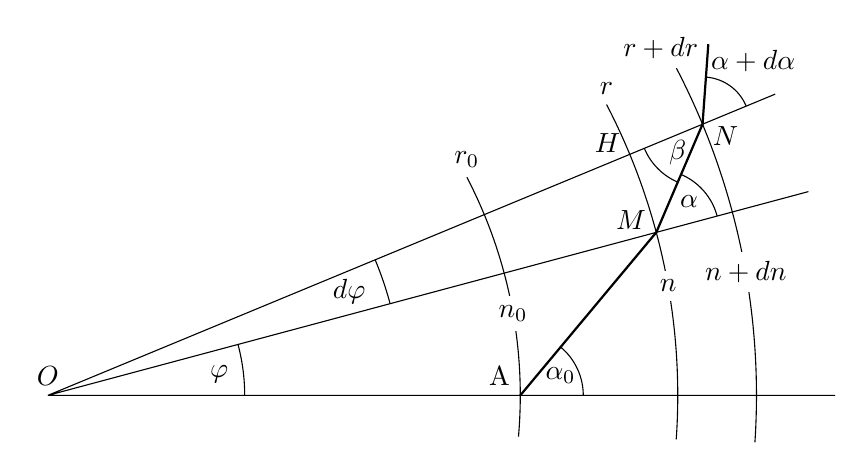
\begin{tikzpicture}
  %radial lines
  \draw (0,0) node[above]{$O$} 
        -- ++(0:10cm)
        (0,0) -- ++(15:10cm)
        (0,0) -- ++(22.5:10cm);
  %Radius r0, r, r + dr      
  \draw ([shift=(-5:6cm)]0,0) arc (-5:27.5:6cm) node [above] {$r_0$}
        ([shift=(-4:8cm)]0,0) arc (-4:27.5:8cm) node [above] {$r$}
        ([shift=(-3.8:9cm)]0,0) arc (-3.8:27.5:9cm) node [above, xshift=-0.2cm] {$r +
        dr$};
  %path of the light
  \draw [thick] (0:6cm) node [above left]{A}
        -- (15:8cm) node [above left, yshift=-0.1cm] {$M$}
        -- (22.5:9cm) node [below right, yshift=0.1cm]{$N$}
        -- (28:9.5cm);
  \draw (22.5:8cm) node [above left, yshift=-0.1cm] {$H$};
  %angles
  \draw ([shift=(-157.5:0.8cm)]22.5:9cm) arc (-157.5:-113.2:0.8cm) node [above,
          yshift=0.1cm]{$\beta$}
        ([shift=(15:0.8cm)]15:8cm) arc (15:66.8:0.8cm) node [below,
          yshift = -0.15cm, xshift=0.1cm]{$\alpha$}
        ([shift=(22.5:0.6cm)]22.5:9cm) arc (22.5:85.9:0.6cm) node
          [xshift=0.6cm, yshift=0.2cm]{$\alpha+d\alpha$}
        ([shift=(0:0.8cm)]0:6cm) arc (0:50.2:0.8cm) node [below,
          yshift=-0.14cm]{$\alpha_0$}
        ([shift=(0:2.5cm)]0,0) arc (0:15:2.5cm) node [below left,
          yshift=-0.15cm]{$\varphi$}
        ([shift=(15:4.5cm)]0,0) arc (15:22.5:4.5cm) node [below left,
          yshift=-0.12cm]{$d\varphi$};
  %refraction rates
  \draw (10:6cm) node[fill=white] {$n_0$}
        (10:8cm) node[fill=white] {$n$}
        (10:9cm) node[fill=white] {$n + dn$};
        
\end{tikzpicture}
\caption{Skizze des Sph"arischen Modells}
\label{fig:13_3}
\end{figure}

W"ahrend diesen Umformungen wurde durch $r'(\varphi)$ geteilt. 
In den folgenden Gleichungen sei Vorausgesetzt, dass $r'(\varphi) \neq 0$. 
Dieser Spezialfall wird im Kapitel \ref{ch:spezialfall_2} behandelt. 

F"ur sehr kleine $d\varphi$ ist $\alpha = \beta$. 
Somit k"onnen wir die Gleichung \ref{eq:13_6} quadrieren und \ref{eq:13_8} einsetzen.

$$\frac{(n \cdot r(\varphi))^2}{\left( \frac{r'(\varphi)}{r(\varphi)} \right)^2 +1} = (r_0 n_0 \sin \alpha_0)^2$$

Diese Gleichung ist eine Differentialgleichung erster Ordnung. 
Jedoch ist erneut der Term $sin^2(\alpha_0)$ vorhanden, welcher von $r'(\varphi_0)$ abhängt. 
Damit die DGL auch korrekte Anfangsbedingungen erhält, leiten wir die Gleichung nach $\varphi$ ab und erhalten:

$$\frac{d}{d\varphi}\left(\frac{(n r)^2}{\left(\frac{r'}{r}\right)^2 + 1}\right) =  \frac{2nr (n'r `+ nr') \left( \left( \frac{r'}{r} \right)^2 +1\right) - (nr)^2 2 \frac{r'' r - r'^2}{r}}{\left( \left( \frac{r'}{r} \right)^2 + 1 \right)^2}$$
$$ = \frac{2nr}{\left( \left( \frac{r'}{r} \right)^2 + 1 \right)^2} \left( (n'r + nr') \left( \left( \frac{r'}{r} \right)^2 + 1 \right) - n \left( r'' r - r'^2 \right) \right) = \frac{d}{d\varphi} \left(\left( r_0 n_0 \sin \alpha_0\right)^2 \right) = 0$$
$$\Rightarrow (n'r + nr') \left( \left( \frac{r'}{r} \right)^2 + 1 \right) = n \left( r'' r - r'^2 \right)$$
$$\Rightarrow \frac{n'r'^2}{r} + \frac{n r'^2}{r^2} + n'r + nr' + nr'^2 = r'' r n$$

\begin{equation}
r'' = \frac{1}{r} \left( n' + r' + r'^2 \left( 1 + \frac{1}{r^2} + \frac{n'}{n r} \right) \right)
\end{equation}

In dieser Herleitung wurde durch $n$ und $r$ geteilt. werden jedoch nie $= 0$ sein.
Deshalb muss hier nicht mehr weiter Eingeschr"ankt werden. 
Nun wird $n'(r(\varphi))$ genauer untersucht. 
Nach der Kettenregel ergibt: $\frac{dn}{d\varphi} = \frac{dn}{dr} \cdot \frac{dr}{d\varphi}$. 
Die Ableitung $\frac{dn}{dr}$ wird im Folgenden als $n'_r$ gekennzeichnet.

$$r'' = \frac{r'}{r} \left( 1 + n'_r + r' \left( 1 + \frac{1}{r^2} + \frac{n'_r r'}{n r}\right) \right)$$

Nun wird die oben verwendete Approximation $n(r) = 1 + \mu e^{-\sigma r}$, $n'_r(r) = -\sigma \mu e^{-\sigma r}$ eingesetzt:

\begin{equation} \label{eq:sphere_dgl_approx}
r'' = \frac{r'}{r} \left(1 - \sigma \mu e^{-\sigma r} + r' \left( 1 + \frac{1}{r^2} - \frac{\sigma \mu e^{-\sigma r}}{r (1 + \mu e^{-\sigma r})} \right) \right)
\end{equation}



%WRONG CALCULATIONS:
% $$\Rightarrow \frac{1}{\left(\frac{r'(\varphi)}{r(\varphi)}\right)^2+1} =
% \left(\frac{r_0 n_0 \sin\alpha_0}{n \cdot r(\varphi)}\right)^2$$
% $$\Rightarrow \left(\frac{r'(\varphi)}{r(\varphi)}\right)^2 = \left(\frac{n \cdot
% r(\varphi)}{r_0 n_0 \sin\alpha_0}\right)^2 - 1$$
% \begin{equation}
% \Rightarrow r'(\varphi)^2 = \left(\frac{n \cdot r(\varphi)^2}{r_0 n_0 \sin
% \alpha_0}\right)^2 - r(\varphi)^2
% \end{equation}
% 
% Wenn nun dieselbe Approximation wie beim planaren Modell f"ur $n(r)=1 + \mu e^{-\sigma r}$
% verwendet wird, l"asst sich die Differentialgleichung nummerisch l"osen, siehe Abbildung
% \ref{fig:13_4}.


% FIGURE: linear solution of wrong ODE
\begin{figure}
\centering
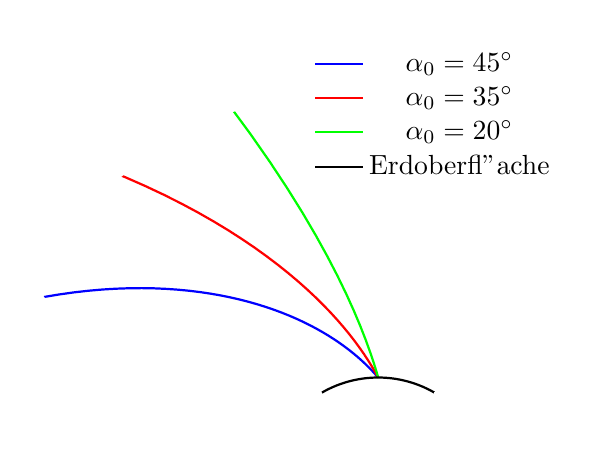
\begin{tikzpicture}
  \begin{polaraxis} [scale=1.5, ticks=none, xmin=60, xmax = 150, ymin=30,
  ymax=180, axis lines* = none, axis line style = {draw=white,line width=0.0001pt},
  grid=none, legend pos = north east, legend style={draw=none}] 

    %alpha = 45Deg
    \addplot [mark = none, thick, color=blue] coordinates {
      (90.00000,50.00000)(91.49972,51.55642)(92.99943,53.16195)(94.49915,54.81814)
      (95.99887,56.52660)(97.49859,58.28896)(98.99830,60.10694)(100.49802,61.98228)
      (101.99774,63.91679)(103.49745,65.91235)(104.99717,67.97087)(106.49689,70.09435)
      (107.99660,72.28484)(109.49632,74.54445)(110.99604,76.87536)(112.49576,79.27982)
      (113.99547,81.76016)(115.49519,84.31878)(116.99491,86.95815)(118.49462,89.68081)
      (119.99434,92.48940)(121.49406,95.38664)(122.99377,98.37533)(124.49349,101.45834)
      (125.99321,104.63868)(127.49293,107.91941)(128.99264,111.30370)(130.49236,114.79483)
      (131.99208,118.39618)(133.49179,122.11122)(134.99151,125.94357)(136.49123,129.89691)
      (137.99094,133.97508)(139.49066,138.18203)(140.99038,142.52182)(142.49010,146.99866)
      (143.98981,151.61687)(145.48953,156.38093)(146.98925,161.29545)(148.48896,166.36518)
      (149.98868,171.59504) };
      
    \addlegendentry{$\alpha_0 = 45^\circ$}
    
    \addplot [mark = none, thick, color=red] coordinates {
      (90.00000,50.00000)(91.49972,52.50858)(92.99943,55.14366)(94.49915,57.91163)
      (95.99887,60.81918)(97.49859,63.87336)(98.99830,67.08156)(100.49802,70.45154)
      (101.99774,73.99147)(103.49745,77.70995)(104.99717,81.61597)(106.49689,85.71900)
      (107.99660,90.02902)(109.49632,94.55647)(110.99604,99.31235)(112.49576,104.30819)
      (113.99547,109.55614)(115.49519,115.06896)(116.99491,120.86003)(118.49462,126.94341)
      (119.99434,133.33390)(121.49406,140.04706)(122.99377,147.09918)(124.49349,154.50741)
      (125.99321,162.28978)(127.49293,170.46523)(128.99264,179.05361)(130.49236,188.07581)
      (131.99208,197.55378)(133.49179,207.51060)(134.99151,217.97045)(136.49123,228.95875)
      (137.99094,240.50225)(139.49066,252.62904)(140.99038,265.36857)(142.49010,278.75179)
      (143.98981,292.81129)(145.48953,307.58128)(146.98925,323.09760)(148.48896,339.39796)
      (149.98868,356.52204) };
      
    \addlegendentry{$\alpha_0 = 35^\circ$}
    
    \addplot[mark = none, thick, color=green] coordinates {
      (90.00000,50.00000)(90.81615,52.57573)(91.63231,55.28349)(92.44846,58.13003)
      (93.26461,61.12246)(94.76433,67.02688)(96.26405,73.49923)(97.76376,80.59427)
      (99.26348,88.37223)(100.76320,96.89922)(102.26292,106.24730)(103.76263,116.49585)
      (105.26235,127.73224)(106.76207,140.05230)(108.26178,153.56044)(109.76150,168.37161)
      (111.26122,184.61232)(112.76093,202.42119)(114.26065,221.94924)(115.76037,243.36267)
      (117.26009,266.84432)(118.75980,292.59455)(120.25952,320.83159)(121.75924,351.79564)
      (123.25895,385.75098)(124.75867,422.98718)(126.25839,463.81974)(127.75811,508.59592)
      (129.25782,557.69781)(130.75754,611.54413)(132.25726,670.59108)(133.75697,735.34081)
      (135.25669,806.34585)(136.75641,884.21170)(138.25612,969.59804)(139.75584,1063.23102)
      (141.25556,1165.90965)(142.75528,1278.50952)(144.25499,1401.98458)(145.75471,1537.38491)
      (147.25443,1685.86590)(147.93799,1758.22138)(148.62155,1833.68275)(149.30512,1912.38330)
      (149.98868,1994.46218) };
      
    \addlegendentry{$\alpha_0 = 20^\circ$}
    
    \addplot +[mark=none, domain=60:120,color=black, samples=360, thick] {50};
    \addlegendentry{Erdoberfl"ache}

  \end{polaraxis}
\end{tikzpicture}
\caption{Nummerische L"osung des Sph"arischen Modells mit der exponentiellen
Approximation (Gleichung: \ref{eq:sphere_dgl_approx})}
\label{fig:13_4}
\end{figure}












